\subsection{Definability}
Up to this point we have neglected schemata containing free variables. We will now correct this oversight. 

Consider the structure $A$ (which should look familiar) defined by
\[
    U^A = [3], L^A=\{\op{1}{2},\op{1}{3}\}
\]
Let $S(x)$ be the schema
\[
    S(x):\ \ \ \neg(\exists y)Lyx.
\]
$S(x)$ picks out $1$ uniquely from the structure $A$, because $1$ is the only element in $U^A$ which does not have an incoming edge. Symbolically, we express this as
\[
\{a\in U^A\mid A\models S[x|a]\}=\{1\}.
\]

$S(x)$ expresses the property of having in-degree zero. Since we only consider properties extensionally, we can also say that, in a given structure, $S(x)$ defines the set of nodes of in-degree zero. The concept of definability is central in logic (and many other disciplines). We enshrine it in a definition.

\begin{definition}
Let $S(x)$ be a schema with one free variable $x$ and let $A$ be a structure.
We define $S[A]=\{a\in U^A\mid A\models S[x|a]\}$. In other words, $S[A]$ is the set of nodes $a \in A$ that satisfy the schema $S(x)$ in $A$ when we assign $a$ to the variable $x$. We call $S[A]$ the \emph{set defined by} $S(x)$ in $A$.
\end{definition}

\begin{definition}
We say a set $V\subseteq U^A$ is a \emph{definable subset of} $A$ if and only if there is a schema $S(x)$ such that $S[A]=V$. We write $\Def{A}$ for the set of definable subsets of $A$.
\end{definition}

Note that the set $\{2,3\}$ is defined by the schema
\[
S'(x):\ \ \ \neg(\exists y)Lxy.
\]

Are either of the sets $\{2\}$ or $\{3\}$ definable as subsets of $A$? Try as you might, you won't find a schema which picks out either $2$ or $3$ individually. Intuitively, this is because the nodes labelled 2 and 3 appear to be ``indistinguishable from a structural point of view''. Backing up this notion of indistinguishability, we see that the function $h$ mapping 1 to 1, 2 to 3, and 3 to 2, is an automorphism of $A$ which happens to exchange $2$ and $3$. The relevance of this to the question of definability is the content of the following fundamental theorem.

%\subsubsection*{The Automorphism Theorem, Orbits, and Definability over finite structures}
\subsubsection*{The Automorphism Theorem}

The following result, known as the Automorphism Theorem, is an important aid in the study of definability. It is a corollary to Theorem \ref{iso-thm}.
\begin{corollary}\label{aut-thm}
Let $A$ be a graph and $h\in\aut{A}$. For every $a\in U^A$ and every schema $S(x)$,
\[
A\models S[x|a]\mbox{ if and only if }A\models S[x|h(a)]. 
\]
\end{corollary}
\begin{aside}
    Show that Corollary \ref{aut-thm} is a corollary to Theorem \ref{iso-thm}
\end{aside}

Corollary \ref{aut-thm} provides a useful necessary condition for a set to be definable in an arbitrary structure, and enables us to give a characterization of the definable subsets of finite structures. 
If $f$ is a function with domain $U$ and $V\subseteq U$, we define $f[V]=\{f(a)\mid a\in V\}$ (the $f$ \emph{image} of $V$). With this notation in hand, we can now state a corollary to Corollary \ref{aut-thm} which bears on definability.
\begin{corollary}\label{aut-def-cor}
Let $A$ be a graph and $h\in\aut{A}$. If $V$ is a definable subset of $A$, then $h[V]=V$.
\end{corollary}
\begin{aside}
    Show that Corollary \ref{aut-def-cor} is a corollary to Corollary \ref{aut-thm}
\end{aside}

Thus, in order to show that $V$ is \emph{not} a definable subset of $A$ it suffices to exhibit an $h\in\aut{A}$ and $a\in V$ such that $h(a)\not\in V$. 
\subsection*{Orbits and Definability over Finite Structures}

In the case of finite structures, the converse of Corollary \ref{aut-def-cor} is true.
\begin{theorem}\label{fin-aut-def-thm}
Let $A$ be a finite graph and $V\subseteq U^A$. $V$ is a definable subset of $A$ if and only if for every $h\in\aut{A}$, $h[V]=V$.
\end{theorem}
In order to prove Theorem \ref{fin-aut-def-thm}, and to apply it to questions of counting definable sets, the following definitions will be useful. 

\begin{definition}
The \emph{orbit of a node} $a\in U^A$ \emph{under the action of} $\aut{A}$ is the set of all possible images of $a$ under actions $f \in \aut{A}$. Symbolically,
\[
\orb{a}{\aut{A}}=\{h(a)\mid h\in\aut{A}\}.
\]
\end{definition}

\begin{definition}
The \emph{orbits of $A$} is the set of all orbits of individual elements $a \in A$. Symbolically:
\[
    \autorbs{A}=\{\orb{a}{\aut{A}}\mid a\in U^A\}
\]
\end{definition}
\textbf{Proof Sketch of Theorem \ref{fin-aut-def-thm}}:
We aim to show that for every finite graph $A$, $V \subset A$ is definable iff every automorphism $h \in \aut{A}$ leaves $V$ unchanged. The generalization to structures interpreting multiple polyadic predicates is straightforward.

First, suppose $A$ is a finite graph, $a\in U^A$, and $V=\orb{a}{\aut{A}}$. We construct a schema $S(x)$ such that $S[A]=V$. We may suppose without loss of generality that $U^A=[k]$ for some $k\in\mathbb{Z}^+$ and that $a=1$. For each $1\leq i,j\leq k$, let the schema $S_{i,j}$ be $Lx_ix_j$ if $\op{i}{j}\in L^A$, and $\neg Lx_ix_j$ otherwise. Let $S(x)$ be the schema
\[
(\exists x_2)\ldots(\exists x_k)(\bigwedge_{1\leq i,j\leq k}S_{i,j}\wedge\bigwedge_{1\leq i<j\leq k}x_i\neq x_j\wedge(\forall y)\bigvee_{1\leq i\leq k} y=x_i).
\] 
Let $a_1,\dots,a_k$ be a sequence of nodes from $U^A$ and observe that
\[
A\models(\bigwedge_{1\leq i,j\leq k}S_{i,j}\wedge\bigwedge_{1\leq i<j\leq k}x_i\neq x_j\wedge(\forall y)\bigvee_{1\leq i\leq k} y=x_i)[(x_1|a_1),\ldots,(x_k|a_k)]
\]
if and only if the function mapping $i$ to $a_i$ is an automorphism of $A$. \qed

As a corollary to Corollary \ref{aut-def-cor} and Theorem \ref{fin-aut-def-thm} we have:
\begin{corollary}\label{def-orbs-cor}
Let $A$ be a finite graph and $V\subseteq U^A$. $V$ is a definable subset of $A$ if and only if either $V=\emptyset$ or there is a sequence of sets $O_1, \ldots,O_k$, where each $O_i\in\autorbs{A}$, and $V = O_1\cup\ldots\cup O_k$.
\end{corollary}

\begin{aside}
    Use Corollary \ref{aut-def-cor} and Theorem \ref{fin-aut-def-thm} to prove this. 
\end{aside}

It follows at once from Corollary \ref{def-orbs-cor}, that if $A$ is a finite graph, then the number of definable subsets of $A$ is $2^{\card{\autorbs{A}}}$. 

\begin{definition}
    We say that a graph $A$ is \emph{rigid} if and only if $\aut{A}=\{e\}$, that is, $A$ has no non-trivial automorphisms.
\end{definition}

It follows at once from Theorem \ref{fin-aut-def-thm} that if $A$ is a finite rigid structure and $V\subseteq U^A$, then $V\in\Def{A}$.

\begin{aside}
    Why? Think about what $\aut{A}=\{e\}$ implies about the orbit of each element (and hence $\autorbs{A}$). 
\end{aside}

\subsubsection*{Automorphisms and Degree}
In applying our analysis of definability over finite structures in terms orbits to particular examples, it will be useful to observe the following connections between automorphisms and degree.
Let $A$ be a graph and $a\in U^A$. Recall that the \emph{neighborhood of} $a$ in $A$ is $\nbh{a}{A} := \{b\in U^A\mid\op{a}{b}\in L^A\}$. The \emph{degree of} $a$ in $A$ is $\dg{a}{A} := \card{\{b\in U^A\mid\op{a}{b}\in L^A\}}$. We have the following fact:
\begin{proposition}
For every graph $A$, $a\in U^A$, and $h\in\aut{A}$,
\[
h[\nbh{a}{A}]=\nbh{h(a)}{A}.
\]
Hence,
\[
\dg{a}{A} = \dg{h(a)}{A}. 
\]
In other words, automorphisms preserve degree. 
\end{proposition}

\begin{aside}
    Show that this follows from the definition of an automorphism.
\end{aside}

\subsubsection*{An example: definable subsets of simple graphs with four nodes}

To make this all a little bit more concrete, let's give a complete analysis of the definable subsets of simple graphs with four nodes. 

We begin by classifying all members of $\modn{\sg}{4}$ up to isomorphism - that is, we exhibit an example of each ``isomorphism-type'' of size-4 simple graph. What does this mean? Recall that for every $A\in\modn{\sg}{4}$, $\orb{A}{\mathbb{S}_4}$ is the set of $B$ such that $B\cong A$. Thus, these orbits correspond to the isomorphism types of structures in $\modn{\sg}{4}$, and we will make a list that includes exactly one structure from each orbit. Another way of putting this is that we make a \emph{succinct} list of structures from $\modn{\sg}{4}$, that is, a maximal length list of such structures, no two of which are isomorphic.
\begin{aside}
In general, if a group $G$ acts on a set $X$, we may define an equivalence relation $\sim$ on $X$ by $a\sim b$ if and only if there is an $f\in G$ such that $fa=b$. The equivalence class $\hat{a}$ of an element $a\in X$ with respect to this equivalence relation is the \emph{orbit of $a$} under this group action, and the equivalence relation is often referred to as the \emph{orbit equivalence relation}. Thus, in the case to hand, the orbit equivalence relation of the action of $\symn{k}$ on  $\modn{\sg}{k}$ we've defined is exactly the isomorphism relation.
\end{aside} 

We already know that $\size{$\modn{\sg}{4}$}= 2^{\binom{4}{2}}=2^6=64$, and though this is not a very large number, nonetheless, it will useful to organize our effort systematically in order to compile a succinct list of simple graphs of size four. If graphs $A$ and $B$ are isomorphic, then they have the same number of edges. Let's write $\gsize{A}$ for the number of undirected edges of a simple graph $A$. We call $\gsize{A}$ the \emph{edge-size} of $A$, in contrast to \size{A}, which is the number of vertices of $A$. For $A\in \modn{\sg}{4}$, $0\leq \gsize{A}\leq 6$. For each of these seven possible edge-sizes, we will make a succinct list of the graphs of that edge-size, and then put them together to get a succinct list of all the simple graphs of size 4. 

A simple observation will  nearly halve our effort in compiling these lists. For a simple graph $A$, we define $A^c$, the \emph{graph complement} of $A$ as follows.
\[ A^c: U^{A^c}= U^A; \op{i}{j}\in E^{A^c}\mbox{ iff } i\neq j \mbox{ and } \op{i}{j}\not\in E^A.\]
If we like, we can visualize a simple graph as having ``solid edges'' (the edges that are included in the graph) and ``transparent edges'' (the edges that are omitted from the graph). Complementation turns the solid edges transparent, and the transparent edges solid, while retaining the loop-free character of the graph. 
\begin{lemma}\label{complement-lem}
For all simple graphs $A$ and $B$ and all functions $f:U^A\mapsto U^B$,
$f$ is an isomorphism from $A$ onto $B$ if and only if $f$ is an isomorphism of $A^c$ onto $B^c$. Hence,
\[
A\cong B \mbox{ iff } A^c\cong B^c,
\]
and for all functions $f:U^A\mapsto U^A$,
\[
f\in\aut{A} \mbox{ iff } f\in\aut{A^c}.
\]
Moreover,
$\card{\orb{A}{\symn{4}}} = \card{\orb{A^c}{\symn{4}}}$, and $\card{\aut{A_i}} = \card{\aut{A_j}}$.
\end{lemma}
\begin{aside}
Prove Lemma \ref{complement-lem}.
\end{aside}
%\begin{aside}
    %Prove that $\aut{A} = \aut{A^c}$ for every simple graph $A$. 

%It follows immediately from Lemma \ref{complement-lem} that if $A_i$ and $A_j$ are complements, we have $\card{\aut{A_i}} = \card{\aut{A_j}}$ and  %This will make our counting easier, because it nearly halves the amount of work we have to do. 
%\end{aside}
It follows immediately from Lemma \ref{complement-lem} that succinct lists of graphs in  $\modn{\sg}{4}$ with edge-size $0\leq i\leq 6$, immediately generate succinct lists with edge-size $6-i$, via complementation. 
Finally, we are prepared to compile our lists.

 There is a single graph in $\modn{\sg}{4}$ with no edges which we will call $A_1$. This looks like

\[
    \begin{array}{|l|}
    \hline
    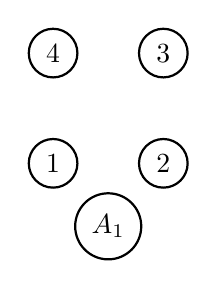
\begin{tikzpicture}
[scale=.2]
\begin{scope}[every node/.style={circle,thick,draw}]
    \node (1) at (0,4) {1};
    \node (2) at (7,4) {2};
    \node (3) at (7,11) {3};
    \node (4) at (0,11) {4};
   \node(A) at (3.5,0) {$A_1$};
\end{scope}
\end{tikzpicture}\\
\hline
\end{array}
\]

By complementation, there is also a single graph with 6 edges.

\[
    \begin{array}{|l|}
    \hline
    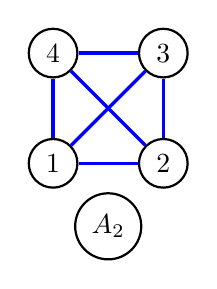
\begin{tikzpicture}
[scale=.2]
\begin{scope}[every node/.style={circle,thick,draw}]
    \node (1) at (0,4) {1};
    \node (2) at (7,4) {2};
    \node (3) at (7,11) {3};
    \node (4) at (0,11) {4};
   \node(A) at (3.5,0) {$A_2$};
\end{scope}

\begin{scope}[%>={Stealth[black]},
              every node/.style={fill=white,circle},
              every edge/.style={draw=blue,very thick}]
     \draw (1) edge  (2);
     \draw (2) edge  (3);
     \draw (3) edge  (4);
     \draw (4) edge  (1);
     \draw (4) edge  (2);
     \draw (3) edge  (1);
             
\end{scope}
\end{tikzpicture}\\
\hline
\end{array}
\]

Up to isomorphism, there is one size-4 graph with a single edge (since we only care about equivalence up to isomorphism, the labels of the ends of the single edge don't matter). By complementation, there is a single size-4 graph with 5 edges. 

\[
    \begin{array}{|l|l|}
        \hline
        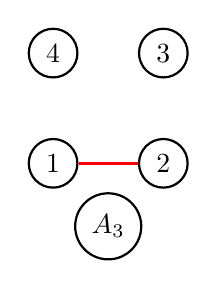
\begin{tikzpicture}
        [scale=.2]
        \begin{scope}[every node/.style={circle,thick,draw}]
            \node (1) at (0,4) {1};
            \node (2) at (7,4) {2};
            \node (3) at (7,11) {3};
            \node (4) at (0,11) {4};
           \node(A) at (3.5,0) {$A_3$};
        \end{scope}

        \begin{scope}[%>={Stealth[black]},
                      every node/.style={fill=white,circle},
                      every edge/.style={draw=red,very thick}]
              \draw (1) edge  (2);
             %\draw (2) edge  (3);
             %\draw (3) edge  (4);
             %\draw (4) edge  (1);
             %\draw (4) edge  (2);
             %\draw (3) edge  (1);             
        \end{scope}
        \end{tikzpicture}
        &
        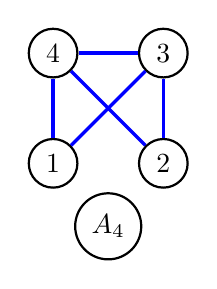
\begin{tikzpicture}
        [scale=.2]
        \begin{scope}[every node/.style={circle,thick,draw}]
            \node (1) at (0,4) {1};
            \node (2) at (7,4) {2};
            \node (3) at (7,11) {3};
            \node (4) at (0,11) {4};
           \node(A) at (3.5,0) {$A_4$};
        \end{scope}

        \begin{scope}[%>={Stealth[black]},
                      every node/.style={fill=white,circle},
                      every edge/.style={draw=blue,very thick}]
             %\draw (1) edge  (2);
             \draw (2) edge  (3);
             \draw (3) edge  (4);
             \draw (4) edge  (1);
             \draw (4) edge  (2);
             \draw (3) edge  (1);
                     
        \end{scope}
        \end{tikzpicture}\\
        \hline
    \end{array}
\]

There are two non-isomorphic size-4 graphs with two edges, and, again by complementation, two such graphs with 4 edges. 

\[
    \begin{array}{|l|l|}
    \hline

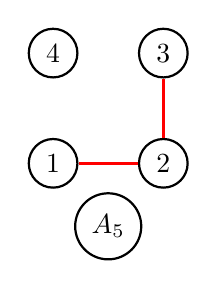
\begin{tikzpicture}
[scale=.2]
\begin{scope}[every node/.style={circle,thick,draw}]
    \node (1) at (0,4) {1};
    \node (2) at (7,4) {2};
    \node (3) at (7,11) {3};
    \node (4) at (0,11) {4};
   \node(A) at (3.5,0) {$A_5$};
\end{scope}

\begin{scope}[%>={Stealth[black]},
              every node/.style={fill=white,circle},
              every edge/.style={draw=red,very thick}]
\draw (1) edge  (2);
     \draw (2) edge  (3);
     %\draw (3) edge  (4);
     %\draw (4) edge  (1);
     %\draw (4) edge  (2);
     %\draw (3) edge  (1);             
\end{scope}
\end{tikzpicture}
&
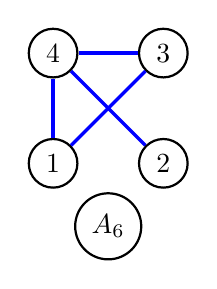
\begin{tikzpicture}
[scale=.2]
\begin{scope}[every node/.style={circle,thick,draw}]
    \node (1) at (0,4) {1};
    \node (2) at (7,4) {2};
    \node (3) at (7,11) {3};
    \node (4) at (0,11) {4};
   \node(A) at (3.5,0) {$A_6$};
\end{scope}

\begin{scope}[%>={Stealth[black]},
              every node/.style={fill=white,circle},
              every edge/.style={draw=blue,very thick}]
%\draw (1) edge  (2);
%     \draw (2) edge  (3);
     \draw (3) edge  (4);
     \draw (4) edge  (1);
     \draw (4) edge  (2);
     \draw (3) edge  (1);
             
\end{scope}
\end{tikzpicture}
\\
\hline
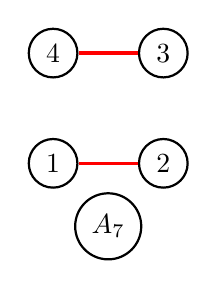
\begin{tikzpicture}
[scale=.2]
\begin{scope}[every node/.style={circle,thick,draw}]
    \node (1) at (0,4) {1};
    \node (2) at (7,4) {2};
    \node (3) at (7,11) {3};
    \node (4) at (0,11) {4};
   \node(A) at (3.5,0) {$A_7$};
\end{scope}

\begin{scope}[%>={Stealth[black]},
              every node/.style={fill=white,circle},
              every edge/.style={draw=red,very thick}]
\draw (1) edge  (2);
     %\draw (2) edge  (3);
     \draw (3) edge  (4);
     %\draw (4) edge  (1);
     %\draw (4) edge  (2);
     %\draw (3) edge  (1);             
\end{scope}
\end{tikzpicture}
&
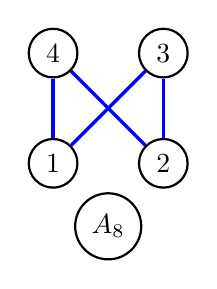
\begin{tikzpicture}
[scale=.2]
\begin{scope}[every node/.style={circle,thick,draw}]
    \node (1) at (0,4) {1};
    \node (2) at (7,4) {2};
    \node (3) at (7,11) {3};
    \node (4) at (0,11) {4};
   \node(A) at (3.5,0) {$A_8$};
\end{scope}

\begin{scope}[%>={Stealth[black]},
              every node/.style={fill=white,circle},
              every edge/.style={draw=blue,very thick}]
%\draw (1) edge  (2);
     \draw (2) edge  (3);
%     \draw (3) edge  (4);
     \draw (4) edge  (1);
     \draw (4) edge  (2);
     \draw (3) edge  (1);
     \end{scope}
\end{tikzpicture}

    \\
    \hline
    \end{array}
\]

Lastly, there are three non-isomorphic size-4 simple graphs with three edges. $A_9$ and $A_{10}$ are complements of each other, whereas $A_{11}$, is isomorphic to its own complement. 

\[
    \begin{array}{|l|l|l|}
    \hline
    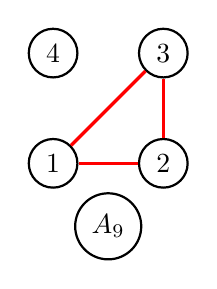
\begin{tikzpicture}
[scale=.2]
\begin{scope}[every node/.style={circle,thick,draw}]
    \node (1) at (0,4) {1};
    \node (2) at (7,4) {2};
    \node (3) at (7,11) {3};
    \node (4) at (0,11) {4};
   \node(A) at (3.5,0) {$A_9$};
\end{scope}

\begin{scope}[%>={Stealth[black]},
              every node/.style={fill=white,circle},
              every edge/.style={draw=red,very thick}]
\draw (1) edge  (2);
     \draw (2) edge  (3);
%     \draw (3) edge  (4);
%     \draw (4) edge  (1);
%     \draw (4) edge  (2);
     \draw (3) edge  (1);
     \end{scope}
\end{tikzpicture}
&
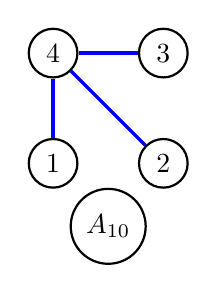
\begin{tikzpicture}
[scale=.2]
\begin{scope}[every node/.style={circle,thick,draw}]
    \node (1) at (0,4) {1};
    \node (2) at (7,4) {2};
    \node (3) at (7,11) {3};
    \node (4) at (0,11) {4};
   \node(A) at (3.5,0) {$A_{10}$};
\end{scope}

\begin{scope}[%>={Stealth[black]},
              every node/.style={fill=white,circle},
              every edge/.style={draw=blue,very thick}]
%\draw (1) edge  (2);
%     \draw (2) edge  (3);
     \draw (3) edge  (4);
     \draw (4) edge  (1);
     \draw (4) edge  (2);
%     \draw (3) edge  (1);
             
\end{scope}
\end{tikzpicture}
&
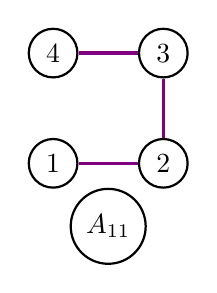
\begin{tikzpicture}
[scale=.2]
\begin{scope}[every node/.style={circle,thick,draw}]
    \node (1) at (0,4) {1};
    \node (2) at (7,4) {2};
    \node (3) at (7,11) {3};
    \node (4) at (0,11) {4};
   \node(A) at (3.5,0) {$A_{11}$};
\end{scope}

\begin{scope}[%>={Stealth[black]},
              every node/.style={fill=white,circle},
              every edge/.style={draw=violet,very thick}]
 \draw (1) edge  (2);
     \draw (2) edge  (3);
     \draw (3) edge  (4);
%     \draw (4) edge  (1);
 %    \draw (4) edge  (2);
  %   \draw (3) edge  (1);
     \end{scope}
\end{tikzpicture}
\\
\hline

\end{array}
\]

\begin{aside}
    Verify that these are all of the non-isomorphic graphs of size 4 by beginning with 4 empty nodes and iteratively constructing all non-isomorphic graphs with increasing number of edges. We will later establish this via application of Theorem \ref{orb-stab-thm}.
\end{aside}

Now that we have a maximal collection of pairwise non-isomorphic graphs in $\modn{\sg}{4}$, we can calculate $\card{\orb{A_i}{\symn{4}}}$ and $\card{\aut{A_i}}$ for each $1\leq i\leq 11$. 

What is $\card{\orb{A_1}{\symn{4}}}$, or in other words, how many distinct ways can we place 0 edges onto 4 labelled nodes? There is only one way to do this, so $\card{\orb{A_1}{\symn{4}}} = 1$. What is $\card{\aut{A_1}}$, or in other words, how many ways can we permute the edges of $A_1$ once the edges are fixed in place? There are no edges, so any permutation of the nodes (of which there are $4! = 24$) is valid. It follows that $\card{\aut{A_1}} = 24$. It follows from Lemma \ref{complement-lem} that $\card{\orb{A_2}{\symn{4}}} = 1$ and $\card{\aut{A_2}} = 24$ as well. 

As another example, let's calculate $\card{\orb{A_5}{\symn{4}}}$ and $\card{\aut{A_5}}$ (and hence the values for $A_6$ as well). There are $4 \cdot 3 = 12$ ways of placing 2 edges onto 4 nodes such that the two edges are connected as in $A_5$, as there are $4$ choices for the ``central'' node and $\binom{3}{2} = 3$ choices for which two other nodes (which we will call \emph{leaves}) get connected to the central node. It follows that $\card{\orb{A_5}{\symn{4}}} = \card{\orb{A_6}{\symn{4}}} = 12$. Once the edges have been fixed, there are two possible automorphisms: the identity automorphism, and the automorphism which exchanges the two leaf nodes. It follows that $\card{\aut{A_5}} = \card{\aut{A_6}} = 2$. 

Without too much extra work, we arrive at the complete table:

\[
\begin{array}{|c|c|c|}
\hline
A_i  & \card{\orb{A_i}{\symn{4}}} & \card{\aut{A_i}}\\
\hline
A_1 & 1 & 24\\
\hline
A_2 & 1 & 24 \\
\hline
A_3 & 6 & 4\\
\hline
A_4 & 6 & 4\\
\hline
A_5 & 12 & 2\\
\hline
A_6 & 12 & 2\\
\hline
A_7 & 3 & 8 \\
\hline
A_8 & 3 & 8 \\
\hline
A_9 & 4 & 6 \\
\hline
A_{10} & 4 & 6 \\
\hline
A_{11} & 12 & 2\\
\hline
\end{array}
\]

\begin{aside}
    Calculate each of the values not discussed in the examples. 
\end{aside}

Note the ``verification'' of the result predicted by the Orbit-Stabilizer Theorem: $\card{\orb{A_i}{\symn{4}}} \cdot \card{\aut{A_i}} = \card{\symn{4}} (= 24)$. Note also that 
\[
\sum_{1\leq i\leq 11}\card{\orb{A_i}{\symn{4}}}=64,
\]
thereby confirming that we have accounted for all structures up to isomorphism!
\begin{aside}
    No member of $\modn{\sg}{4}$ is rigid, as each has non-trivial automorphisms. This suggests an interesting question: ``what is the least $n$ such that $\modn{\sg}{n}$ contains a rigid graph?''
\end{aside}
%\subsection{Addendum}

By Corollary \ref{def-orbs-cor}, calculating $\autorbs{A_i}$ suffices to determine which sets are definable in each $A_i$. 

\begin{example}
What is $\autorbs{A_5}$?
\end{example}
To determine $\autorbs{A_5}$, it suffices to determine the orbits of individual elements. The orbit of node $4$ is $\{4\}$, as it is the only isolated node. The orbit of $2$ is $\{2\}$, as it is the only node of degree two. The orbit of $1$ is $\{1, 3\}$ as $1$ is a leaf node, and we had an automorphism that exchanged leaf nodes. As the set of orbits partition the nodes, the orbit of $3$ is $\{1, 3\}$ as well. It follows that $\autorbs{A_5} = \{\{2\}, \{4\}, \{1, 3\}\}$. 

\begin{aside}
A \emph{partition} of a set $S$ is a collection $\mathcal{P}$ of subsets of $S$ such that: (1) every $s \in S$ is in some $P \in \mathcal{P}$, and (2) if $P, P' \in \mathcal{P}$ and $P \cap P' \neq 0$, then $P = P'$ (ie, no distinct elements of $\mathcal{P}$ overlap).

$\autorbs{A}$ trivially satisfies condition (1), since every node in $A$ is in its own orbit. Complete the proof $\autorbs{A}$ is a partition of the nodes of $A$ by showing that condition (2) holds. 
\end{aside}  

With a little more work, we arrive at the following table. 
\[
\begin{array}{l l}
A_i & \autorbs{A_i}\\
\hline
A_1, A_2 & \{[4]\}\\
A_3, A_4 & \{\{1,2\},\{3,4\}\}\\
A_5, A_6 & \{\{2\},\{4\},\{1,3\}\}\\
A_7, A_8 & \{[4]\}\\
A_9, A_{10} & \{\{1,2,3\},\{4\}\}\\
A_{11} & \{\{1,4\},\{2,3\}\}
\end{array}
\]

\begin{aside}
    Derive each of the above sets of orbits yourself, to make sure all the concepts fit into place. 
\end{aside}
\newpage
\iffalse
\subsection*{Proofs for Theorem \ref{aut-thm} and Theorem \ref{fin-aut-def-thm}}
We now develop the necessary technology in order to give proof sketches for Theorem \ref{aut-thm} and Theorem \ref{fin-aut-def-thm}.  

\subsubsection*{Automorphisms and Degree}
Let $A$ be a graph and $a\in U^A$. Recall that the \emph{neighborhood of} $a$ in $A$ is $\nbh{a}{A} := \{b\in U^A\mid\op{a}{b}\in L^A\}$. The \emph{degree of} $a$ in $A$ is $\dg{a}{A} := \card{\{b\in U^A\mid\op{a}{b}\in L^A\}}$. We have the following fact:
\begin{proposition}
For every graph $A$, $a\in U^A$, and $h\in\aut{A}$,
\[
h[\nbh{a}{A}]=\nbh{h(a)}{A}.
\]
Hence,
\[
\dg{a}{A} = \dg{h(a)}{A}. 
\]
In other words, automorphisms preserve degree. 
\end{proposition}

\begin{aside}
    Show that this follows from the definition of an automorphism.
\end{aside}

\begin{definition}
    We say that a graph $A$ is \emph{rigid} if and only if $\aut{A}=\{e\}$, that is, $A$ has no non-trivial automorphisms.
\end{definition}

It follows at once from Theorem \ref{fin-aut-def-thm} that if $A$ is a finite rigid structure and $V\subseteq U^A$, then $V\in\Def{A}$.

\begin{aside}
    Why? Think about what $\aut{A}=\{e\}$ implies about the orbit of each element (and hence $\autorbs{A}$). 
\end{aside}

\begin{aside}
    No member of $\modn{\sg}{4}$ is rigid, as each has non-trivial automorphisms. This suggests an interesting question: ``what is the least $n$ such that $\modn{\sg}{n}$ contains a rigid graph?''
\end{aside}

\subsubsection*{Proof Sketch of Theorem \ref{fin-aut-def-thm}}
We aim to show that for every finite graph $A$, $V \subset A$ is definable iff every automorphism $h \in \aut{A}$ leaves $V$ unchanged. The generalization to structures interpreting multiple polyadic predicates is straightforward.

First, suppose $A$ is a finite graph, $a\in U^A$, and $V=\orb{A}{\aut{A}}$. We construct a schema $S(x)$ such that $S[A]=V$ by . We may suppose without loss of generality that $U^A=[k]$ for some $k\in\mathbb{Z}^+$ and that $a=1$. For each $1\leq i,j\leq k$, let the schema $S_{i,j}$ be $Lx_ix_j$ if $\op{i}{j}\in L^A$, and $\neg Lx_ix_j$ otherwise. Let $S(x)$ be the schema
\[
(\exists x_2)\ldots(\exists x_k)(\bigwedge_{1\leq i,j\leq k}S_{i,j}\wedge\bigwedge_{1\leq i<j\leq k}x_i\neq x_j\wedge(\forall y)\bigvee_{1\leq i\leq k} y=x_i).
\] 
Let $a_1,\dots,a_k$ be a sequence of nodes from $U^A$ and observe that
\[
A\models(\bigwedge_{1\leq i,j\leq k}S_{i,j}\wedge\bigwedge_{1\leq i<j\leq k}x_i\neq x_j\wedge(\forall y)\bigvee_{1\leq i\leq k} y=x_i)[(x_1|a_1),\ldots,(x_k|a_k)]
\]
if and only if the function mapping $i$ to $a_i$ is an automorphism of $A$. \qed


Theorem \ref{aut-thm} is a corollary of the following more general result concerning isomorphisms of structures.
\iffalse
\begin{theorem}\label{iso-thm}
Suppose $A$ and $B$ are structures and $f$ is an isomorphism of $A$ onto $B$. Then for every schema $S(x_1,\ldots,x_k)$ and sequence of elements $a_1,\dots,a_k\in U^A$,
\begin{equation}\label{iso-eq}
A\models S[(x_1|a_1),\ldots,(x_k|a_k)]\mbox{ iff }B\models S[(x_1|f(a_1)),\ldots,(x_k|f(a_k))].
\end{equation}
\end{theorem}

{\bf Proof sketch of Theorem \ref{iso-thm}}:
We give the argument for graphs; the generalization to structures interpreting multiple polyadic predicates is straightforward.
The argument proceeds by induction on the syntactic structure of schemata. The base case verifies (\ref{iso-eq}) for atomic schemata, that is, schemata of the form $Lx_ix_j$ or $x_i=x_j$, for some $i,j$. In this case, the verification follows directly from the hypothesis that $f$ is an isomorphism from $A$ onto $B$, in particular, that it is edge-preserving and injective.

Suppose $S$ is a truth-functional combination, for example the conjunction, of schemata $S'$ and $S''$, where, as hypothesis of induction, (\ref{iso-eq}) holds for both $S'$ and $S''$. Then,
\[
\begin{array}{lc}
A\models S[(x_1|a_1),\ldots,(x_k|a_k)] & \mbox{ iff}\\
A\models S'[(x_1|a_1),\ldots,(x_k|a_k)]\mbox{ and }A\models S''[(x_1|a_1),\ldots,(x_k|a_k)] & \mbox{ iff}\\
B\models S'[(x_1|f(a_1)),\ldots,(x_k|f(a_k))]\mbox{ and }B\models S''[(x_1|f(a_1)),\ldots,(x_k|f(a_k))] & \mbox{ iff}\\
B\models S[(x_1|f(a_1)),\ldots,(x_k|f(a_k))].
\end{array}
\]
The first and third biconditionals follow from the truth-functional semantics of conjunction, while the second follows from the induction hypothesis.

Finally, suppose that $S$ is $(\exists y)S'(x_1,\ldots,x_k,y)$ and (\ref{iso-eq}) holds for $S'$ (the universal quantifier is handled similarly). Then,
\[
\begin{array}{lc}
A\models S[(x_1|a_1),\ldots,(x_k|a_k)] & \mbox{ iff}\\
\mbox{for some $a\in U^A$ }
A\models S'[(x_1|a_1),\ldots,(x_k|a_k),(y|a)] & \mbox{ iff}\\
\mbox{for some $a\in U^A$ }
B\models S'[(x_1|f(a_1)),\ldots,(x_k|f(a_k)),(y|f(a))] & \mbox{ iff}\\
\mbox{for some $b\in U^B$ }
B\models S'[(x_1|f(a_1)),\ldots,(x_k|f(a_k)),(y|b)] & \mbox{ iff}\\
B\models S[(x_1|f(a_1)),\ldots,(x_k|f(a_k))].
\end{array}
\]
The first and fourth biconditionals follow from the semantics for the existential quantifier, the second from the induction hypothesis, and the third from the hypothesis that $f$ is an isomorphism from $A$ onto $B$, in particular, that it is
surjective. \qed 

\begin{aside}
    In the proof above, the only truth-functional connective we considered was conjunction. The other cases are handled similarly. Complete those cases yourself, either by writing out the whole argument, or by showing that a conditional can be defined in terms of some conditionals whose cases you already worked out (for example, each of the connectives can be defined in terms of $\lnot$ and $\land$, so those two cases suffice). 
\end{aside}
\fi
\begin{aside}
    Show that Theorem \ref{aut-thm} is a corollary to Theorem \ref{iso-thm}
\end{aside}
\fi
\subsection*{Definability in Infinite Structures}

As we've just seen, Corollary \ref{aut-thm} leads to a complete analysis of the definable subsets of finite structures - they are exactly those sets invariant under the action of the automorphism group of the structure. In the case of infinite structures, Corollary \ref{aut-thm} still provides a useful necessary condition for definability, and in some cases leads to a complete analysis of definability. But there are many infinite structures for which this is no longer the case, and other methods are required to achieve a satisfactory understanding of definability. We explore two very different examples in this section.
%We now turn away from the safe confines of the finite and present two examples pertaining to definability in infinite structures.

\subsubsection*{A Structure With Many Automorphisms: The Integers with Absolute Value}
Let $A$ be the infinite graph defined by
\[
    U^A = \mathbb{Z}, L^A = \{\op{i}{j}\mid j \mbox{ is the absolute value of } i\}
\]
(Recall that the absolute value of an integer $i$ is $i$, if $i\geq 0$, and is $-i$, if $i< 0$.) 

\begin{center}
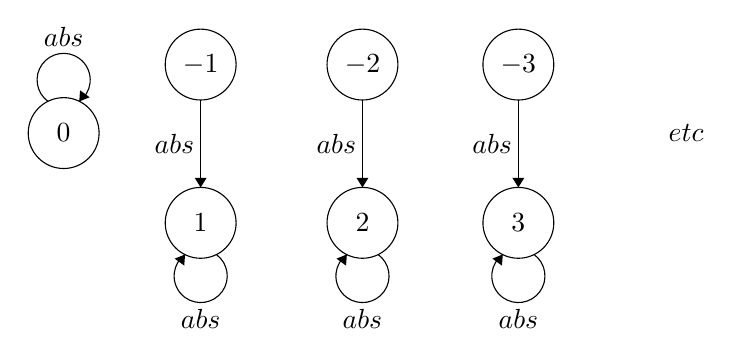
\begin{tikzpicture}[scale=0.15]
\tikzstyle{every node}+=[inner sep=0pt]
\draw [black] (14.4,-29.1) circle (3);
\draw (14.4,-29.1) node {$0$};
\draw [black] (26,-23.3) circle (3);
\draw (26,-23.3) node {$-1$};
\draw [black] (26,-36.7) circle (3);
\draw (26,-36.7) node {$1$};
\draw [black] (39.7,-23.3) circle (3);
\draw (39.7,-23.3) node {$-2$};
\draw [black] (39.7,-36.7) circle (3);
\draw (39.7,-36.7) node {$2$};
\draw [black] (52.9,-23.3) circle (3);
\draw (52.9,-23.3) node {$-3$};
\draw [black] (52.9,-36.7) circle (3);
\draw (52.9,-36.7) node {$3$};
% \draw [black] (67.1,-29.1) circle (3);
\node at (67.1,-29.1) {$etc$};
\draw [black] (13.077,-26.42) arc (234:-54:2.25);
\draw (14.4,-21.85) node [above] {$abs$};
\fill [black] (15.72,-26.42) -- (16.6,-26.07) -- (15.79,-25.48);
\draw [black] (26,-26.3) -- (26,-33.7);
\fill [black] (26,-33.7) -- (26.5,-32.9) -- (25.5,-32.9);
\draw (25.5,-30) node [left] {$abs$};
\draw [black] (27.323,-39.38) arc (54:-234:2.25);
\draw (26,-43.95) node [below] {$abs$};
\fill [black] (24.68,-39.38) -- (23.8,-39.73) -- (24.61,-40.32);
\draw [black] (39.7,-26.3) -- (39.7,-33.7);
\fill [black] (39.7,-33.7) -- (40.2,-32.9) -- (39.2,-32.9);
\draw (39.2,-30) node [left] {$abs$};
\draw [black] (41.023,-39.38) arc (54:-234:2.25);
\draw (39.7,-43.95) node [below] {$abs$};
\fill [black] (38.38,-39.38) -- (37.5,-39.73) -- (38.31,-40.32);
\draw [black] (54.223,-39.38) arc (54:-234:2.25);
\draw (52.9,-43.95) node [below] {$abs$};
\fill [black] (51.58,-39.38) -- (50.7,-39.73) -- (51.51,-40.32);
\draw [black] (52.9,-26.3) -- (52.9,-33.7);
\fill [black] (52.9,-33.7) -- (53.4,-32.9) -- (52.4,-32.9);
\draw (52.4,-30) node [left] {$abs$};
\end{tikzpicture}
\end{center}


Every permutation $g$ of $\mathbb{Z}^+$ can be extended to an automorphism $h$ of $A$ by setting $h(i)=g(i)$, for $i\in \mathbb{Z}^+$; $h(0)=0$; and $h(i)=-g(-i)$, for $i<0$. 

\begin{aside}
    Why is this? The only relation we have in our graph is the absolute-value relation, so our graph looks like a bunch of pairs $n, -n$ (for $n$ positive) where there is an edge from $-n$ to $n$ and an edge from $n$ to $n$ (ie a self-loop at $n$), plus $0$ all on its own with a self-loop. So long as we keep $0$ fixed in place, permuting any of our $(n, -n)$-pairs gives us an automorphism, provided that we match don't ``flip'' any of the pairs, that is, negative numbers (which have in-degree 0) map to negative numbers, and positive numbers (which have in-degree 2) map to positive numbers. The definition given above ensures this. 
\end{aside}



Let's write $\mathbb{Z}^-$ for the set of negative integers. Thus, $\autorbs{A}= \{\mathbb{Z}^+,\{0\},\mathbb{Z}^-\}$. Each orbit of $\aut{A}$ acting on $U^A$ is definable:
\begin{itemize}
\item 
$S_1[A] = \mathbb{Z}^+$, where $S_1(x)$ is $(\exists y)(y\neq x \wedge Lyx)$;
\item 
$S_2[A] = \mathbb{Z}^-$, where $S_2(x)$ is $(\forall y)\neg Lyx$;
\item 
$S_3[A] = \{0\}$, where $S_3(x)$ is $\neg S_1(x)\wedge\neg S_2(x)$.
\end{itemize} 

\begin{aside}
    $S_1[A] = \mathbb{Z}^+$ as the positive integers are the only ones which have in-neighbours distinct from themselves (because there is an edge from a negative integer to its positive absolute value). Explain in your own words why $S_2[A] = \mathbb{Z}^-$ and $S_3[A] = \{0\}$. 
\end{aside}

By Corollary \ref{def-orbs-cor}, it follows that there are exactly eight sets definable in $A$:
\begin{enumerate}
\item $\emptyset$,
\item $\{0\}$,
\item $\mathbb{Z}^+$,
\item $\mathbb{Z}^-$,
\item $\mathbb{Z}^+\cup\mathbb{Z}^-$,
\item $\mathbb{Z}^+\cup\{0\}$,
\item $\mathbb{Z}^-\cup\{0\}$,
\item $\mathbb{Z}$.
\end{enumerate}
\iffalse
\subsubsection*{Defining Infinite Graphs Themselves}
We've just figured out which subsets of $A$ are definable, but what about $A$ itself - ie, can $A$ be uniquely specified by some schema?

The situation would be simpler if we had a finite graph.
\begin{theorem}
If $D$ is a finite graph, then there is a schema $S$ such that for every graph $D'$, 
\[
D'\models S \mbox{ if and only if } D'\cong D.
\]
\end{theorem}

\begin{aside}
    Give a proof of this theorem. Intuitively, the idea is that if a graph is finite, you only need to specify finitely many things about it (eg how many nodes there are, which nodes are connected by edges) in order to uniquely pick out the graph. 
\end{aside}

In sharp contrast, the following theorem shows that \emph{no} infinite structure can be perfectly described by any schema. In order to state the result, we need to define $\theo{D}$, the \emph{complete theory of} $D$:
\[
\theo{D} = \{S\mid S \mbox{ is a schema and } D\models S\}. 
\]
\begin{theorem}\label{infnotcat-thm}
For every infinite graph $D$, there is a graph $D'$, $D'\models\theo{D}$ and $D'\not\cong D$.
\end{theorem}
Theorem \ref{infnotcat-thm} is a corollary to the Compactness Theorem for PQT, a fundamental\footnote{By many accounts, this is \emph{the} most fundamental result about First-Order Logic (the common name for what we call PQT).} result we will study shortly.
\fi
\subsubsection*{A Rigid Structure: The Natural Numbers with Successor}
We now look at another infinite structure $B$ where definability behaves very differently. $B$ is described by:
\[
    U^B = \mathbb{N}, L^B = \{\op{i}{j}\mid j=i+1\}
\]

\begin{center}
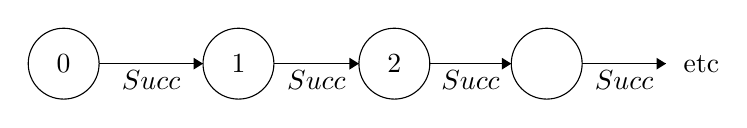
\begin{tikzpicture}[scale=0.15]
\tikzstyle{every node}+=[inner sep=0pt]
\draw [black] (12,-29.5) circle (3);
\draw (12,-29.5) node {$0$};
\draw [black] (26.8,-29.5) circle (3);
\draw (26.8,-29.5) node {$1$};
\draw [black] (40,-29.5) circle (3);
\draw (40,-29.5) node {$2$};
\draw [black] (52.9,-29.5) circle (3);
% \draw (52.9,-29.5) node {$3$};
\node at (66,-29.5) {etc};
\draw [black] (15,-29.5) -- (23.8,-29.5);
\fill [black] (23.8,-29.5) -- (23,-29) -- (23,-30);
\draw (19.4,-30) node [below] {$Succ$};
\draw [black] (29.8,-29.5) -- (37,-29.5);
\fill [black] (37,-29.5) -- (36.2,-29) -- (36.2,-30);
\draw (33.4,-30) node [below] {$Succ$};
\draw [black] (43,-29.5) -- (49.9,-29.5);
\fill [black] (49.9,-29.5) -- (49.1,-29) -- (49.1,-30);
\draw (46.45,-30) node [below] {$Succ$};
\draw [black] (55.9,-29.5) -- (63,-29.5);
\fill [black] (63,-29.5) -- (62.2,-29) -- (62.2,-30);
\draw (59.45,-30) node [below] {$Succ$};
\end{tikzpicture}
\end{center}

A first observation is that $\aut{B}=\{e\}$, that is, $B$ is a rigid structure. Intuitively, any automorphism must map $0$ to itself, since it is the only element which doesn't have anything less than it. Similarly, any automorphism must map any positive $n$ to itself, since $n$ is the only number with exactly $n - 1$ predecessors. 

We can establish this formally by mathematical induction. Suppose $h$ is an automorphism of $B$. Since $0$ is the only node of $B$ with in-degree $0$, we must have $h(0)=0$. Now suppose, as induction hypothesis, that $h(n)=n$. Since $n+1$ is the only member of $U^B$ to which $n$ is related, it follows from the hypothesis that $h$ is an automorphism that $h(n+1)=n+1$. It follows that for all $k\in U^B$, $h(k)=k$. Hence, $\aut{B}=\{e\}$. 

This argument suggests that for every $k\in U^B$, $\{k\}$ is definable over $B$. Let's show this, again by induction. First, the schema $S^0(x): (\forall y)\neg Lyx$ defines $\{0\}$ over $B$. Next, as induction hypothesis, suppose that $S^n(x)$ defines $\{n\}$ over $B$. Let $z$ be a variable which does not occur anywhere in $S^n(x)$ and let $S^n(z)$ be the result of replacing $x$ with $z$ at all its occurrences in $S^n(x)$. Then the schema $(\exists z)(S^n(z)\wedge Lzx)$ defines $\{n+1\}$ over $B$. This completes the induction and establishes that for every $k\in U^B$, $\{k\}$ is definable over $B$. It follows at once that every finite subset of $U^B$ and every co-finite subset of $U^B$ is definable over $B$. 

\begin{aside}
    Why is it important that $z$ be a variable which occurs nowhere in $S^n(x)$?
\end{aside}

What other subsets of $U^B$ are definable over $B$? Note that since $B$ is rigid, there is no possibility of exhibiting an automorphism $h$ of $B$ with $h[X]\neq X$, that is, the ``automorphism method'' is powerless to establish the undefinability of any subset of $U^B$ in $B$. Could it be that every subset of $U^B$ is definable over $B$? 
\iffalse
\subsubsection*{Defining Infinite Graphs Themselves}
We've just figured out which subsets of $A$ are definable, but what about $A$ itself - ie, can $A$ be uniquely specified by some schema?

The situation would be simpler if we had a finite graph.
\begin{theorem}
If $D$ is a finite graph, then there is a schema $S$ such that for every graph $D'$, 
\[
D'\models S \mbox{ if and only if } D'\cong D.
\]
\end{theorem}

\begin{aside}
    Give a proof of this theorem. Intuitively, the idea is that if a graph is finite, you only need to specify finitely many things about it (eg how many nodes there are, which nodes are connected by edges) in order to uniquely pick out the graph. 
\end{aside}

In sharp contrast, the following theorem shows that \emph{no} infinite structure can be perfectly described by any schema. In order to state the result, we need to define $\theo{D}$, the \emph{complete theory of} $D$:
\[
\theo{D} = \{S\mid S \mbox{ is a schema and } D\models S\}. 
\]
\begin{theorem}\label{infnotcat-thm}
For every infinite graph $D$, there is a graph $D'$, $D'\models\theo{D}$ and $D'\not\cong D$.
\end{theorem}
Theorem \ref{infnotcat-thm} is a corollary to the Compactness Theorem for PQT, a fundamental\footnote{By many accounts, this is \emph{the} most fundamental result about First-Order Logic (the common name for what we call PQT).} result we will study shortly.
\fi


